\documentclass[12pt,a4paper]{article}

% Packages
\usepackage[utf8]{inputenc}
\usepackage[T1]{fontenc}
\usepackage{geometry}
\usepackage{graphicx}
\usepackage{hyperref}
\usepackage{enumitem}
\usepackage{xcolor}
\usepackage{tikz}
\usepackage{booktabs}
\usepackage{fancyhdr}
\usepackage{tcolorbox}
\usepackage{listings}
\usepackage{amsmath}
\usepackage{amssymb}
\usepackage{longtable}

% Page geometry
\geometry{margin=2.5cm}

% Colors
\definecolor{primaryblue}{RGB}{0, 102, 204}
\definecolor{successgreen}{RGB}{40, 167, 69}
\definecolor{dangerred}{RGB}{220, 53, 69}
\definecolor{warningyellow}{RGB}{255, 193, 7}
\definecolor{lightgray}{RGB}{248, 249, 250}
\definecolor{codegray}{RGB}{45, 45, 45}
\definecolor{codegreen}{RGB}{0, 128, 0}
\definecolor{purple}{RGB}{128, 0, 128}

% TikZ libraries
\usetikzlibrary{shapes, arrows, positioning, fit, backgrounds, calc}

% Listings setup
\lstset{
    basicstyle=\ttfamily\small,
    backgroundcolor=\color{lightgray},
    frame=single,
    framerule=0pt,
    breaklines=true,
    showstringspaces=false,
    keywordstyle=\color{primaryblue}\bfseries,
    commentstyle=\color{codegreen},
    stringstyle=\color{dangerred},
    numbers=left,
    numberstyle=\tiny\color{gray},
    numbersep=5pt,
    xleftmargin=15pt
}

% Header and footer
\pagestyle{fancy}
\fancyhf{}
\fancyhead[L]{\textbf{CS2113 -- Software Development Project}}
\fancyhead[R]{Lecture 4: Sprint 2}
\fancyfoot[C]{\thepage}

% Tcolorbox styles
\tcbuselibrary{skins, breakable, listings}

\newtcolorbox{keyinsight}{
    colback=primaryblue!10,
    colframe=primaryblue,
    title=\textbf{Key Insight},
    fonttitle=\bfseries,
    breakable
}

\newtcolorbox{warning}{
    colback=dangerred!10,
    colframe=dangerred,
    title=\textbf{Warning},
    fonttitle=\bfseries,
    breakable
}

\newtcolorbox{tip}{
    colback=successgreen!10,
    colframe=successgreen,
    title=\textbf{Tip},
    fonttitle=\bfseries,
    breakable
}

\newtcolorbox{definitionbox}{
    colback=lightgray,
    colframe=black!50,
    breakable
}

\newtcolorbox{commandbox}{
    colback=codegray!10,
    colframe=codegray,
    breakable
}

% Title
\title{
    \vspace{-1cm}
    \textbf{Sprint 2: REST APIs and Frontend Development}\\
    \large Lecture 4 Notes\\[0.5cm]
    \normalsize School of Computing Communication and Media Studies
}
\author{Masoud Hamad}
\date{CS2113 -- Software Development Project\\Academic Year 2025}

\begin{document}

\maketitle
\tableofcontents
\newpage

%============================================================
\section{Sprint Retrospective}
%============================================================

\begin{definitionbox}
The \textbf{Retrospective} is a Scrum event where teams discuss process issues and develop solutions. It occurs after the Sprint Review, concluding the current Sprint.
\end{definitionbox}

\subsection{Retrospective Principles}

\begin{itemize}
    \item All team members discuss process challenges openly
    \item Every voice must be heard
    \item Solutions should be concrete actions implementable during the upcoming Sprint
    \item Previously identified issues shouldn't resurface in the next Retrospective
\end{itemize}

\subsection{Mad, Sad, Glad Technique}

Team members categorize their Sprint experiences:

%------------------------------------------------------------
% Figure 1: Mad Sad Glad
%------------------------------------------------------------
\begin{figure}[htbp]
\centering
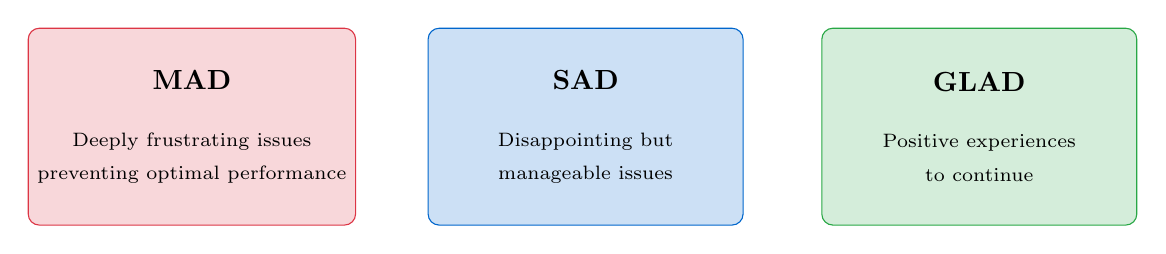
\begin{tikzpicture}[
    card/.style={rectangle, draw, rounded corners, minimum width=4cm, minimum height=2.5cm, align=center}
]
    \node[card, fill=dangerred!20, draw=dangerred] (mad) at (0, 0) {
        \textbf{MAD}\\[0.3cm]
        \scriptsize Deeply frustrating issues\\
        \scriptsize preventing optimal performance
    };

    \node[card, fill=primaryblue!20, draw=primaryblue] (sad) at (5, 0) {
        \textbf{SAD}\\[0.3cm]
        \scriptsize Disappointing but\\
        \scriptsize manageable issues
    };

    \node[card, fill=successgreen!20, draw=successgreen] (glad) at (10, 0) {
        \textbf{GLAD}\\[0.3cm]
        \scriptsize Positive experiences\\
        \scriptsize to continue
    };
\end{tikzpicture}
\caption{Mad, Sad, Glad Retrospective Categories}
\label{fig:mad-sad-glad}
\end{figure}

\textbf{Examples:}
\begin{itemize}
    \item \textbf{Mad:} ``Spring Boot application won't start on my computer''
    \item \textbf{Sad:} ``Daily Scrum meetings take too long''
    \item \textbf{Glad:} ``Team communication was transparent''
\end{itemize}

\subsection{Retrospective Process}

\begin{enumerate}
    \item Team members independently write cards for each category (no discussion yet)
    \item Review all cards category by category
    \item Identify highest-priority issues from Mad and Sad categories
    \item Develop at least one concrete action per issue
    \item Document actions on the retrospective board
\end{enumerate}

%============================================================
\section{REST APIs}
%============================================================

\subsection{Traditional vs REST Approach}

\textbf{Traditional Web Application:}
\begin{enumerate}
    \item User opens page in browser
    \item Browser requests resource from server
    \item Controller processes request
    \item Controller retrieves data from database
    \item HTML page is generated
    \item HTML response sent to browser
\end{enumerate}

\textbf{REST API Approach:}
\begin{itemize}
    \item Instead of HTML, serialize Java objects to \textbf{JSON format}
    \item Easier consumption by different clients (web, mobile, etc.)
    \item Clear separation between frontend and backend
\end{itemize}

%------------------------------------------------------------
% Figure 2: REST Architecture
%------------------------------------------------------------
\begin{figure}[htbp]
\centering
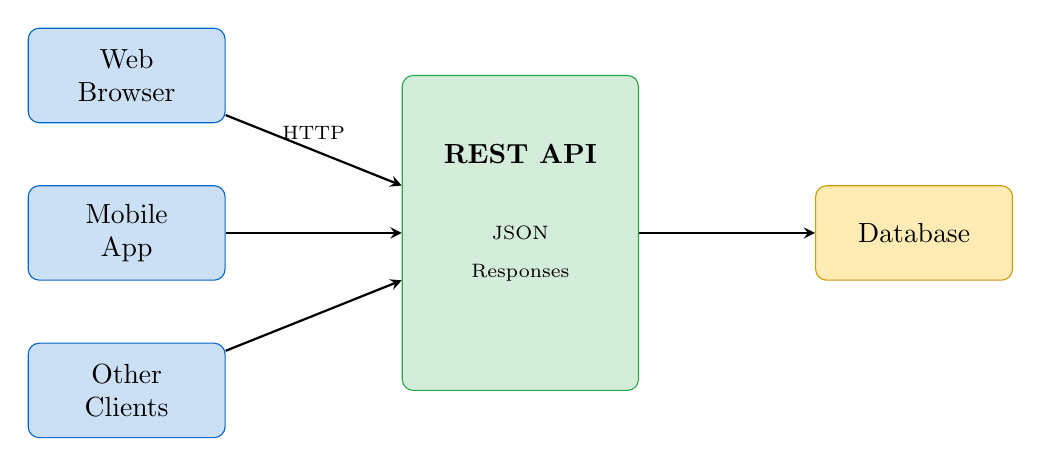
\begin{tikzpicture}[
    node distance=1.5cm,
    component/.style={rectangle, draw=primaryblue, fill=primaryblue!20, rounded corners, minimum width=2.5cm, minimum height=1.2cm, align=center},
    arrow/.style={->, thick, >=stealth}
]
    % Clients
    \node[component] (web) at (0, 2) {Web\\Browser};
    \node[component] (mobile) at (0, 0) {Mobile\\App};
    \node[component] (other) at (0, -2) {Other\\Clients};

    % REST API
    \node[component, minimum width=3cm, minimum height=4cm, fill=successgreen!20, draw=successgreen] (api) at (5, 0) {};
    \node[font=\bfseries] at (5, 1) {REST API};
    \node[font=\scriptsize] at (5, 0) {JSON};
    \node[font=\scriptsize] at (5, -0.5) {Responses};

    % Database
    \node[component, fill=warningyellow!30, draw=warningyellow!80!black] (db) at (10, 0) {Database};

    % Arrows
    \draw[arrow] (web) -- node[above, font=\scriptsize] {HTTP} (api);
    \draw[arrow] (mobile) -- (api);
    \draw[arrow] (other) -- (api);
    \draw[arrow] (api) -- (db);
\end{tikzpicture}
\caption{REST API Architecture}
\label{fig:rest-architecture}
\end{figure}

\subsection{RESTful API Characteristics}

\begin{itemize}
    \item \textbf{Stateless:} Each request contains all information needed
    \item \textbf{Client-Server Separation:} Frontend and backend are independent
    \item \textbf{Resource-Based Paths:} URLs represent resources
    \item \textbf{HTTP Method Semantics:} Methods indicate actions
\end{itemize}

%============================================================
\section{HTTP Methods}
%============================================================

\begin{table}[htbp]
\centering
\begin{tabular}{llp{6cm}}
\toprule
\textbf{Method} & \textbf{Action} & \textbf{Description} \\
\midrule
GET & Read & Retrieve data without modification \\
POST & Create & Create new database entries \\
PUT & Update & Update existing entries \\
DELETE & Remove & Delete database entries \\
\bottomrule
\end{tabular}
\caption{HTTP Methods and Their Actions}
\label{tab:http-methods}
\end{table}

\subsection{RESTful Endpoints Convention}

\begin{table}[htbp]
\centering
\begin{tabular}{llp{5cm}}
\toprule
\textbf{Method} & \textbf{Path} & \textbf{Description} \\
\midrule
GET & /api/quizzes & List all quizzes \\
GET & /api/quizzes/\{id\} & Get quiz by ID \\
POST & /api/quizzes & Create new quiz \\
PUT & /api/quizzes/\{id\} & Update quiz \\
DELETE & /api/quizzes/\{id\} & Delete quiz \\
GET & /api/quizzes/\{id\}/questions & Get quiz questions \\
\bottomrule
\end{tabular}
\caption{RESTful Endpoint Examples}
\label{tab:endpoints}
\end{table}

\begin{keyinsight}
Resource collections use \textbf{plural nouns} (e.g., ``quizzes'' not ``quiz''). Path variables like \texttt{\{id\}} identify specific resources.
\end{keyinsight}

%============================================================
\section{REST Controller Implementation}
%============================================================

\subsection{Basic REST Controller}

\begin{commandbox}
\begin{lstlisting}[language=Java]
@RestController
@RequestMapping("/api")
@CrossOrigin(origins = "*")
public class QuizRestController {

    @Autowired
    private QuizRepository quizRepository;

    @GetMapping("/quizzes")
    public List<Quiz> getAllQuizzes() {
        return quizRepository.findAll();
    }

    @GetMapping("/quizzes/{id}")
    public Quiz getQuizById(@PathVariable Long id) {
        return quizRepository.findById(id)
            .orElseThrow(() -> new ResponseStatusException(
                HttpStatus.NOT_FOUND,
                "Quiz with id " + id + " does not exist"
            ));
    }
}
\end{lstlisting}
\end{commandbox}

\subsection{POST Endpoint with Validation}

\begin{commandbox}
\begin{lstlisting}[language=Java]
@PostMapping("/quizzes")
public Quiz createQuiz(
        @Valid @RequestBody CreateQuizDto quiz,
        BindingResult bindingResult) {

    if (bindingResult.hasErrors()) {
        throw new ResponseStatusException(
            HttpStatus.BAD_REQUEST,
            bindingResult.getAllErrors()
                .get(0).getDefaultMessage()
        );
    }

    Quiz newQuiz = new Quiz(
        quiz.getName(),
        quiz.getDescription()
    );
    return quizRepository.save(newQuiz);
}
\end{lstlisting}
\end{commandbox}

%============================================================
\section{DTO Pattern (Data Transfer Objects)}
%============================================================

\begin{definitionbox}
\textbf{DTO (Data Transfer Object)} is a pattern using dedicated classes to control request/response body format. DTOs prevent undesired attribute updates and hide sensitive information.
\end{definitionbox}

\subsection{Request DTO Example}

\begin{commandbox}
\begin{lstlisting}[language=Java]
public class CreateQuizDto {
    @NotBlank(message = "Name is required")
    private String name;

    @Size(max = 500, message = "Description too long")
    private String description;

    private String courseCode;

    // Constructors, getters, setters
}
\end{lstlisting}
\end{commandbox}

\subsection{Response DTO Example}

\begin{commandbox}
\begin{lstlisting}[language=Java]
public class QuizResultDto {
    private Long questionId;
    private String questionText;
    private String questionDifficulty;
    private int totalAnswers;
    private int correctAnswers;
    private int wrongAnswers;

    // Constructors, getters, setters
}
\end{lstlisting}
\end{commandbox}

%------------------------------------------------------------
% Figure 3: DTO Pattern
%------------------------------------------------------------
\begin{figure}[htbp]
\centering
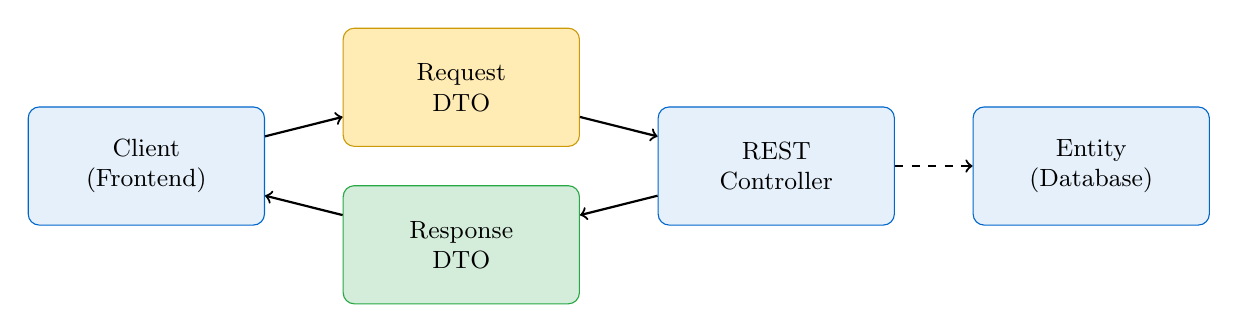
\begin{tikzpicture}[
    node distance=1cm,
    box/.style={rectangle, draw=primaryblue, fill=primaryblue!10, rounded corners, minimum width=3cm, minimum height=1.5cm, align=center, font=\small},
    arrow/.style={->, thick}
]
    \node[box] (client) at (0, 0) {Client\\(Frontend)};
    \node[box, fill=warningyellow!30, draw=warningyellow!80!black] (req) at (4, 1) {Request\\DTO};
    \node[box] (controller) at (8, 0) {REST\\Controller};
    \node[box, fill=successgreen!20, draw=successgreen] (res) at (4, -1) {Response\\DTO};
    \node[box] (entity) at (12, 0) {Entity\\(Database)};

    \draw[arrow] (client) -- (req);
    \draw[arrow] (req) -- (controller);
    \draw[arrow] (controller) -- (res);
    \draw[arrow] (res) -- (client);
    \draw[arrow, dashed] (controller) -- (entity);
\end{tikzpicture}
\caption{DTO Pattern in REST APIs}
\label{fig:dto-pattern}
\end{figure}

%============================================================
\section{HTTP Status Codes}
%============================================================

\subsection{Status Code Ranges}

\begin{itemize}
    \item \textbf{200--299:} Successful responses
    \item \textbf{400--499:} Client errors
    \item \textbf{500--599:} Server errors
\end{itemize}

\subsection{Common Status Codes}

\begin{table}[htbp]
\centering
\begin{tabular}{lp{8cm}}
\toprule
\textbf{Code} & \textbf{Meaning} \\
\midrule
200 OK & Request successful \\
201 Created & Resource created successfully \\
400 Bad Request & Invalid request (e.g., validation error) \\
401 Unauthorized & User not authenticated \\
403 Forbidden & User lacks authorization \\
404 Not Found & Resource not found \\
500 Internal Server Error & Server-side error \\
\bottomrule
\end{tabular}
\caption{Common HTTP Status Codes}
\label{tab:status-codes}
\end{table}

\subsection{ResponseEntity for Custom Responses}

\begin{commandbox}
\begin{lstlisting}[language=Java]
@PostMapping("/quizzes")
public ResponseEntity<?> createQuiz(
        @Valid @RequestBody CreateQuizDto quiz,
        BindingResult bindingResult) {

    if (bindingResult.hasErrors()) {
        return ResponseEntity
            .status(HttpStatus.BAD_REQUEST)
            .body(bindingResult.getAllErrors());
    }

    Quiz newQuiz = new Quiz(quiz.getName());
    quizRepository.save(newQuiz);

    return ResponseEntity
        .status(HttpStatus.CREATED)
        .body(newQuiz);
}
\end{lstlisting}
\end{commandbox}

%============================================================
\section{Swagger API Documentation}
%============================================================

\begin{definitionbox}
\textbf{Swagger} automatically generates API documentation from controller classes using the OpenAPI standard format.
\end{definitionbox}

\subsection{Adding Spring Doc Dependency}

\begin{commandbox}
\begin{lstlisting}[language=XML]
<dependency>
    <groupId>org.springdoc</groupId>
    <artifactId>springdoc-openapi-starter-webmvc-ui</artifactId>
    <version>2.3.0</version>
</dependency>
\end{lstlisting}
\end{commandbox}

\subsection{Access URLs}

\begin{itemize}
    \item JSON format: \texttt{http://localhost:8080/v3/api-docs}
    \item User-friendly UI: \texttt{http://localhost:8080/swagger-ui/index.html}
\end{itemize}

\subsection{Documentation Annotations}

\begin{commandbox}
\begin{lstlisting}[language=Java]
@Tag(name = "Quizzes",
     description = "Operations for quiz management")
@RestController
@RequestMapping("/api/quizzes")
public class QuizRestController {

    @Operation(
        summary = "Get quiz by ID",
        description = "Returns the quiz with the provided ID"
    )
    @ApiResponses(value = {
        @ApiResponse(responseCode = "200",
            description = "Quiz retrieved successfully"),
        @ApiResponse(responseCode = "404",
            description = "Quiz not found")
    })
    @GetMapping("/{id}")
    public Quiz getQuizById(@PathVariable Long id) {
        // ...
    }
}
\end{lstlisting}
\end{commandbox}

%============================================================
\section{Frontend-Backend Communication}
%============================================================

\subsection{Fetch API - GET Request}

\begin{commandbox}
\begin{lstlisting}[language=JavaScript]
fetch("http://localhost:8080/api/quizzes")
    .then(response => response.json())
    .then(quizzes => {
        console.log(quizzes);
    });
\end{lstlisting}
\end{commandbox}

\subsection{Fetch API - POST Request}

\begin{commandbox}
\begin{lstlisting}[language=JavaScript]
fetch("http://localhost:8080/api/quizzes", {
    method: "POST",
    headers: {
        "Accept": "application/json",
        "Content-Type": "application/json"
    },
    body: JSON.stringify({
        name: "JavaScript Quiz",
        description: "Test your JS knowledge"
    })
})
.then(response => response.json())
.then(newQuiz => {
    console.log(newQuiz);
});
\end{lstlisting}
\end{commandbox}

\subsection{Service Function Pattern}

\begin{commandbox}
\begin{lstlisting}[language=JavaScript]
const BACKEND_URL = "http://localhost:8080";

export function getAllQuizzes() {
    return fetch(`${BACKEND_URL}/api/quizzes`)
        .then(response => response.json());
}

export function createQuiz(quiz) {
    return fetch(`${BACKEND_URL}/api/quizzes`, {
        method: "POST",
        headers: {
            "Accept": "application/json",
            "Content-Type": "application/json"
        },
        body: JSON.stringify(quiz)
    })
    .then(response => {
        if (!response.ok) {
            throw new Error("Failed to create quiz");
        }
        return response.json();
    });
}
\end{lstlisting}
\end{commandbox}

%------------------------------------------------------------
% Figure 4: Full Stack Communication
%------------------------------------------------------------
\begin{figure}[htbp]
\centering
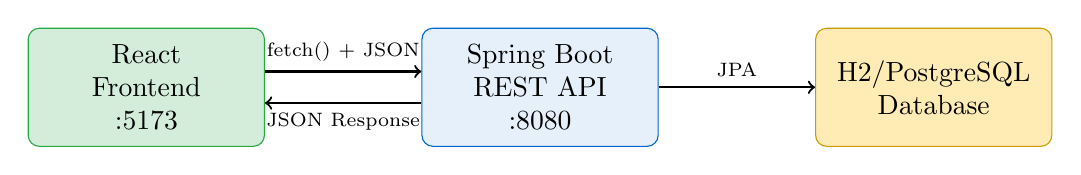
\begin{tikzpicture}[
    node distance=1cm,
    box/.style={rectangle, draw=primaryblue, fill=primaryblue!10, rounded corners, minimum width=3cm, minimum height=1.5cm, align=center},
    arrow/.style={->, thick}
]
    \node[box, fill=successgreen!20, draw=successgreen] (react) at (0, 0) {React\\Frontend\\:5173};
    \node[box] (api) at (5, 0) {Spring Boot\\REST API\\:8080};
    \node[box, fill=warningyellow!30, draw=warningyellow!80!black] (db) at (10, 0) {H2/PostgreSQL\\Database};

    \draw[arrow] ([yshift=0.2cm]react.east) -- node[above, font=\scriptsize] {fetch() + JSON} ([yshift=0.2cm]api.west);
    \draw[arrow] ([yshift=-0.2cm]api.west) -- node[below, font=\scriptsize] {JSON Response} ([yshift=-0.2cm]react.east);
    \draw[arrow] (api) -- node[above, font=\scriptsize] {JPA} (db);
\end{tikzpicture}
\caption{Full Stack Application Communication}
\label{fig:fullstack}
\end{figure}

%============================================================
\section{Data Model Documentation}
%============================================================

Document your data model in README.md using Mermaid syntax:

\begin{commandbox}
\begin{lstlisting}
## Data Model

```mermaid
erDiagram
    QUIZ ||--o{ QUESTION : contains
    QUESTION ||--o{ ANSWER_OPTION : has
    QUIZ }o--|| CATEGORY : belongs_to

    QUIZ {
        Long id
        String name
        String description
        String courseCode
        Boolean published
        LocalDateTime createdAt
    }

    QUESTION {
        Long id
        String text
        String difficulty
    }
```
\end{lstlisting}
\end{commandbox}

%============================================================
\newpage
\section{Exercises}
%============================================================

\begin{tcolorbox}[colback=warningyellow!10, colframe=warningyellow!80!black, title=\textbf{Sprint 2 Deadline}]
All work must be pushed to GitHub repository before the Sprint deadline.
\end{tcolorbox}

\subsection{Exercise 1: Retrospective}
Conduct a Mad-Sad-Glad retrospective using Flinga. Document the board link in README.md.

\subsection{Exercise 2: Select New Scrum Master}
Choose a different team member as Scrum Master for Sprint 2.

\subsection{Exercise 3: Close Sprint 1 Issues}
Close completed Sprint 1 issues and create Sprint 2 milestone.

\subsection{Exercise 4: Create Labels}
Create ``frontend'' and ``backend'' labels for categorizing issues.

\subsection{Exercise 5: User Story Issues}
Create issues for Sprint 2 user stories with appropriate labels and milestone.

\subsection{Exercises 6--9: Task Planning}
Break down each Sprint 2 user story into technical tasks.

\subsection{Exercise 10: Data Model Documentation}
Create entity relationship diagram using Mermaid syntax in README.md.

\subsection{Exercises 11--17: REST Endpoint Implementation}
Implement REST endpoints for:
\begin{itemize}
    \item Get quiz by ID
    \item Get quiz questions
    \item Create answer submission
    \item Get quiz results
    \item Get all categories
    \item Get category by ID
    \item Get category quizzes
\end{itemize}

\subsection{Exercise 18: Swagger Documentation}
\begin{itemize}
    \item Add Spring Doc dependency
    \item Add @Operation annotations to all endpoints
    \item Add @ApiResponses for success/error responses
    \item Group endpoints using @Tag
    \item Add Swagger link to README.md
\end{itemize}

\subsection{Exercises 19--24: Frontend Development}
Plan and implement frontend user stories for student dashboard.

\subsection{Exercise 25: Deploy Frontend}
Deploy frontend application to production (e.g., Render).

\subsection{Exercise 26: Developer Guide}
Update README.md with frontend startup instructions and technology stack.

\subsection{Exercise 27: Create Release}
Create GitHub release ``Sprint 2'' with feature description.

\subsection{Exercise 28: Sprint Review Preparation}
Prepare working demo of both teacher and student dashboards.

%============================================================
\vspace{1cm}
\hrule
\vspace{0.3cm}
\begin{center}
\small
\textit{This document is licensed under Creative Commons BY-NC-SA 4.0}
\end{center}

\end{document}
